\section{壹、前言}

\subsection{一、研究動機}

近年來,物件追蹤技術被廣泛應用於球類運動上,例如鷹眼系統(Hawk-Eye)已被應用於網球、羽球等運動,以追蹤和記錄球的路徑。然而由於其架設成本高,多數運動員無法負擔。為了解決此問題,國立交通大學網路最佳化實驗室開發了深度學習架構 TrackNet,可以由一般攝影機拍攝之網球比賽影片追蹤網球軌跡。(鍾奉原,2020)

排球在我校是非常興盛的一種運動,經常舉辦班際球賽等排球比賽,因此我們便想利用 TrackNetV2 追蹤排球比賽影片中的排球,以協助分析排球比賽,減少人工花費大量時間觀看的成本。

\subsection{二、研究目的}

應用 TrackNetV2 追蹤由一般攝影機(非高速攝影機)所錄製之排球比賽影片中的排球,藉由自動追蹤球的路徑協助排球比賽的賽事分析。

\subsection{三、文獻回顧}

傳統影像物件辨識是根據物件的外顯特徵和統計特徵進行偵測的,但排球比賽中的排球會因打擊的關係而導致有變形的情況出現,再加上移動速度過快,快門相對於球的速度來說較慢,因此容易有影像殘留及模糊的現象出現。

\begin{itemize}
    \setlength\parindent{2em}
    \item []
    \textbf{(一)TrackNet}

    TrackNet(黃昱銓,2018)提出了一個以 CNN(Convolutional Neural Network,卷積神經網路)為基礎的深度學習架構(如圖1)。但不同於其他深度學習網路,它容許一次輸入多張連續幀,可從中學習球的影像特徵及軌跡特性。然後仿效 FCN(FullyConvolutional Network,全卷積網路)的生成階段,生成用於偵測及定位球的熱度圖(如圖2)。最後再依據熱度圖計算畫面中可能存在的網球。這個模型不僅能從模糊影像中定位球的存在,更可以進一步的判斷受遮擋的網球位置,可以很好的達到我們的需求。

    \begin{figure}
        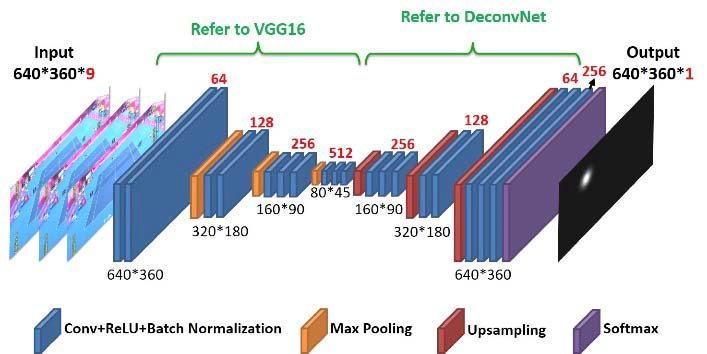
\includegraphics[width = 9cm]{picture/TrackNet 架構圖.jpg}\\
        \caption{、TrackNet 架構圖}
        \label{TrackNet 架構圖}
        
        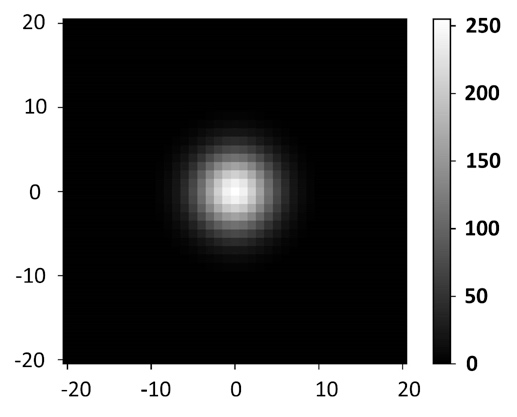
\includegraphics[width = 9cm]{picture/熱度圖.jpg}
        \caption{、熱度圖}
        \label{熱度圖}
    \end{figure}
\end{itemize}

\section{貳、研究設備與器材}

\section{參、研究過程或方法}

\section{肆、研究結果}

\section{伍、討論}

\section{陸、結論}

\section{柒、參考文獻資料}
\begin{itemize}
    \item [一、] 10 程式中(2021 年10 月6 日)。[Day 24] 機器學習- 不能忽視的過擬合與欠擬
    合。檢自:\url{https://ithelp.ithome.com.tw/articles/10278254}
\end{itemize}